\documentclass[
	paper=a4,				% Papierformat
	twoside=true,			% Zweiseitiges Layout
	BCOR=6mm,				% Rand zum Binden
	fontsize=12pt,			% Schriftgröße
	pagesize=auto,			% Schreibt die Papiergröße korrekt ins Ausgabedokument
	numbers=noenddot,		% Kein Punkt nach der Kapitel-Nummer
	bibliography=totoc,		% Quellenverzeichnis im Inhaltsverzeichnis auflisten
	draft=false
]{scrartcl}
% siehe http://tex.stackexchange.com/questions/183149/cant-silence-a-pdftex-pdf-inclusion-multiple-pdfs-with-page-group-error
\pdfsuppresswarningpagegroup=1
% Legt die Zeichenkodierung fest, z.B UTF8
\usepackage[utf8]{inputenc}
% Erweiterten Zeichensatz für europäische Sprachen aktivieren
\usepackage[T1]{fontenc}
% Silbentrennung nach neuer deutscher Rechtschreibung
\usepackage[ngerman]{babel}
% Beseitigt Probleme mit noch nicht vollständig aktualisierten Paketen (z.B. listings)
\usepackage{scrhack}
% Zum flexiblen Einbinden von Grafiken, pdftex ist optional
\usepackage[pdftex]{graphicx}
% Umgebung um mehrere Abbildungen zu einer zu kombinieren
\usepackage{subfig}
% Führt die SCfigure-Umgebung ein (Caption neben der Abbildung)
\usepackage{sidecap}
\renewcommand{\sidecaptionrelwidth}{2.0}
% Damit kann ein Bild vom Text umflossen werden
\usepackage{wrapfig}
% Darstellung für Caption s.u.
\usepackage[font=small,labelfont=bf,labelsep=colon,format=plain]{caption}
\usepackage{amsmath}
\usepackage{amssymb}
\usepackage{cite}
% Verbessert die Kompatibilität von siunitx mit microtype
\usepackage{textcomp}
\usepackage{siunitx}
\sisetup{
	output-decimal-marker = {,},
	per-mode = symbol,
	list-final-separator = { und },
	list-pair-separator = { und },
	range-phrase = { bis },
}
\usepackage{listings}
% Umlaute in Listings sind nur mit folgender Option möglich:
\lstset{
    literate={ö}{{\"o}}1
    {ä}{{\"a}}1
    {ü}{{\"u}}1
}
% Standard-Werte für Listings festlegen:
\lstset{
    frame=single,
    flexiblecolumns=true,
    commentstyle=\color{darkgreen},
    float,
    basicstyle=\small\sffamily,
    numbers=left,
    numberstyle=\tiny,
    showstringspaces=false,
    keepspaces,
    tabsize=4
}
% Zum Einfärben von Code:
\usepackage{color}
\definecolor{darkgreen}{rgb}{0,0.5,0}

% Fußnoten formatieren und Unterstützung für aufeinander folgende Fußnoten:
\usepackage[flushmargin,multiple]{footmisc}
% Hurenkinder und Schusterjungen komplett verbieten:
%\clubpenalty = 10000
%\widowpenalty = 10000
%\displaywidowpenalty = 10000
%\usepackage{microtype}
% Hyperlinks erstellen, wobei Fußnoten aus Kompatibilitätsgründen ausgenommen werden:
\usepackage[hyperfootnotes=false,pdfpagelabels]{hyperref}

% subsubsections werden nummeriert (Standard: subsections)
\setcounter{secnumdepth}{\subsubsectionnumdepth}

% Platz für 3 stellige Seitenzahlen im Inhaltsverzeichnis schaffen:
\makeatletter
\renewcommand{\@pnumwidth}{3em} 
\renewcommand{\@tocrmarg}{4em}
\makeatother

% Schriftgröße der Bildunterschriften verkleinern:
\addtokomafont{caption}{\small\linespread{1}\selectfont}
% Zweite Zeile der Bildunterschrift einrücken:
\setcapindent{1em}

\begin{document}	

\author{Michael Entrup}
\title{Anhang F \\ ImageJ}
\date{April 2017}

\maketitle

% Inhaltsverzeichnis
\tableofcontents

\section{Eine Einführung zu ImageJ}

ImageJ ist ein in Java geschriebenes Programm zur wissenschaftlichen Bildverarbeitung. Auf der Website des Programms (\url{https://imagej.nih.gov}) heißt es \glqq Image Processing and Analysis in Java\grqq. ImageJ wird von einem ehemaligen Mitarbeiter des National Institutes of Health entwickelt, Wayne Rasband. Der Quellcode unterliegt nicht dem Urheberrecht, sondern ist unter \glqq Public Domain\grqq\  freigegeben \cite{rasband_imagej_2004}.

Mit ImageJ2 entsteht im Moment eine neue Version, welche auf die Verarbeitung und Analyse von mehrdimensionalen Datensätzen ausgelegt ist. ImageJ2 ist trotzdem vollständig zu ImageJ1 kompatibel. Dies wird dadurch erreicht, dass die grafische Oberfläche von ImageJ2 weiterhin Zugriff auf alle Funktionen von ImageJ1 gewährt. Abbildung \ref{fig:ImageJ_main} zeigt einen Screenshot von ImageJ. Die neue Programm-Logik von ImageJ2 -- ImgLib2 genannt -- ist vollständig von der grafisch Oberfläche entkoppelt, so dass man sie mit anderer Software nutzen kann. So ist es möglich Plugins zu schreiben, die auch von anderer Software aus dem SciJava-Projekt genutzt werden können. ImageJ2 und damit auch ImgLib2 sind noch nicht fertiggestellt, weshalb in dieser Arbeit ausschließlich mit Programmcode für ImageJ1 gearbeitet wird. Ausgeführt wird der Code jedoch in ImageJ2, bzw. Fiji. Letzteres wird im folgenden Abschnitt erklärt.

\begin{figure}
	\centering
	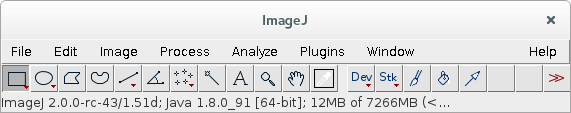
\includegraphics[width=1\linewidth]{Bilder/ImageJ_main}
	\caption{Das Hauptfenster von ImageJ (Debian Linux mit Gnome3). In der Statusleiste ist zu erkennen, dass ImageJ2 in der Version 2.0.0-rc-43 vorliegt und ImageJ1 in der Version 1.51d.}
	\label{fig:ImageJ_main}
\end{figure}

\section{Fiji Is Just ImageJ}

Neben ImageJ existiert die Distribution Fiji. Auf der Website\footnote{\url{http://imagej.net/Fiji}} heißt es dazu: \glqq Fiji is an image processing package—a ``batteries-included'' distribution of ImageJ, bundling a lot of plugins which facilitate scientific image analysis.\grqq\ Das bedeutet, dass neben den Grundfunktionen eine Vielzahl von Plugins vorinstalliert sind. Außerdem hat man Zugriff auf diverse Java-Bibliotheken, wie z.\,B. Apache Commons Math.

Aus Fiji stammen außerdem mehrere Funktionen, die mittlerweile Bestandteil von ImageJ sind. Mit Hilfe des Updaters erhält man automatisch Aktualisierungen für Plugins und ImageJ selbst. Der Script-Editor ermöglicht ein komfortables Schreiben von Macros und Scripten, dank Syntax-Hervorhebung und einer einfachen Auto-Vervollständigung.

Der Updater bietet noch eine besondere Funktion. Man kann eigene Update-Sites hinzufügen und erhält auf diese Weise Aktualisierungen zu Plugins, welche nicht Bestandteil von Fiji sind. Jeder Nutzer kann außerdem seine eigenen Update-Sites auf dem Webserver von ImageJ erstellen und damit die selbst geschriebenen Plugins der Allgemeinheit zur Verfügung stellen. Dieses Verfahren wird auch für das Plugin EFTEMj genutzt. Eine Anleitung zum Hinzufügen von EFTEMj zu ImageJ ist auf der GitHub-Website zum Plugin zu finden.\footnote{\url{https://github.com/m-entrup/EFTEMj}}

\section{ImageJ durch eigene Programme erweitern}

Ein großer Vorteil von ImageJ ist die Erweiterbarkeit. Eine Vielzahl von verfügbaren Plugins\footnote{\url{https://imagej.nih.gov/ij/plugins/}} verdeutlicht, dass diese Erweiterbarkeit von vielen genutzt wird \cite{collins_imagej_2007}. Diese einfache Möglichkeit neue Funktionen zu ergänzen beschränkt sich nicht nur auf Plugins, sondern es ist außerdem möglich Macros und Scripte zu schreiben. Durch das Wegfallen des Kompilierens sind Macros und Scripte sehr einfach zu nutzen. Besonders das Schreiben eines ersten Scriptes gestaltet sich als sehr einfach, da man aus einer von acht Programmier- bzw. Scriptsprachen\footnote{BeanShell, Clojure, Groovy, JavaScript, Python, R, Ruby und Scala (Stand: 29.06.2016)} (8 bei Fiji, 6 bei ImageJ) wählen kann und zusätzlich mit Hilfe des Macro-Recorders passende Code-Schnipsel präsentiert bebommt.

\subsection*{Macros für ImageJ schreiben}

\begin{figure}
	\centering
	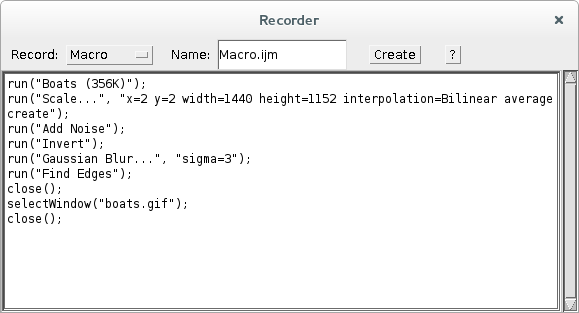
\includegraphics[width=1\linewidth]{Bilder/ImageJ_Macro_Recorder}
	\caption{Der Macro Recorder von ImageJ. Es wurden diverse Bearbeitungsschritte an einem Bild ausgeführt, zu denen der Recorder die entsprechenden Macro-Befehle auflistet.}
	\label{fig:ImageJ_Macro_Recorder}
\end{figure}

Macros eignen sich besonders gut um Abläufe zu automatisieren. Dazu startet man den Macro-Recorder \textbf{[Plugins > Macros > Record\ldots]} und führt die gewünschten Bearbeitungs- und Auswertungsschritte mit ImageJ aus. Im Textfeld des Macro-Recorders erscheint zu jeder genutzten Funktion ein Befehl der Form \texttt{run(''Find Edges'')}. Lässt sich die Funktion durch Parameter anpassen, so sind auch diese im ausgegebenen Befehl enthalten, z.\,B.\ \texttt{run(''Gaussian Blur...'', ''sigma=3'')}. Abbildung \ref{fig:ImageJ_Macro_Recorder} zeigt den Macro Recorder, nachdem schon mehrere Bearbeitungsschritte mit ImageJ ausgeführt wurden. Ein Klick auf \textbf{Create} öffnet den Script-Editor und zeigt die aufgenommen Befehle an\footnote{Alternativ kann man den Script-Editor über den Menü-Eintrag \textbf{[Plugins > Macro > New]} öffnen.}. Mit Hilfe der Anleitung zur ImageJ Macro Sprache (\url{https://imagej.nih.gov/ij/developer/macro/macros.html}) kann man die einzelnen Befehle durch das Hinzufügen von Schleifen und Kontrollstrukturen zu einem erstes, komplexeren Macro erweitern. Viele Funktionen lassen sich mit Hilfe der Macro-Recorders nicht erfassen, weshalb die Website \url{https://imagej.nih.gov/ij/developer/macro/functions.html} all diese Funktionen aufführt, die zusätzlich zur Verfügung stehen. Die Liste wird laufend aktualisiert und führt zu vielen Funktionen hilfreiche Beispiele auf.

Listing \ref{lst:Macro-Beispiel} zeigt ein einfaches Macro, mit dessen Hilfe man den Mittelwert aller Bilder in einem Stack auf 1 normiert. Die \texttt{run()}-Befehle wurden vom Macro-Recorder generiert und anschließend durch String-Verkettung flexibler gestaltet. Die Kommentare, welche mit \texttt{\#} anfangen erklären die einzelnen Schritte innerhalb des Macros.

\begin{figure}
	\lstinputlisting[language=Perl,caption={Ein einfaches Macro für ImageJ},label={lst:Macro-Beispiel}]{Code/NormalizeStack.ijm}
\end{figure}

\subsection*{Einschränkungen von ImageJ Macros}

Viele Aufgaben lassen sich sehr gut mit Hilfe von Macros lösen. Es gibt jedoch Aufgaben, für welche das Schreiben eines Macros nicht sinnvoll ist. Für gewöhnlich führt man mit den \texttt{run()}-Befehlen Funktionen so aus, wie es auch mit Hilfe der grafischen Oberfläche möglich ist. Häufig werden dabei neue Fenster geöffnet. Dabei kann es problematisch sein, dass die Befehle immer auf dem aktuell gewählten Bild ausgeführt wird. Möchte man ein anderes Bild nutzen, so muss man dieses über eine von zwei verfügbaren Methoden machen:

\begin{itemize}
	\item Auswahl des Fensters mit Hilfe des Titels (\texttt{selectWindow("name")}), wobei es zu Problemen bei Namen mit Sonderzeichen kommen kann,
	\item Auswahl des Fensters mit Hilfe der eindeutigen ID (\texttt{selectImage(id)}).
\end{itemize}

In diesem Moment sollte man über die Nutzung einer Script-Sprache Nachdenken, da diese Bilder als Objekte zwischengespeichert werden können.

Beim Ausführen von Macros sollte man nicht dem Computer interagieren. Aktiviert man versehentlich ein falsches Bild, führt dies zu einem Fehler bei der Ausführung des Macros, oder zu einem falschen Ergebnis.

Ein weiter Nachteil von Macros ist die geringe Ausführungsgeschwindigkeit. Dies hängt damit zusammen, dass Änderungen an Bildern direkt ein Update des Bild-Fensters auslösen. Die Aktualisierung der grafischen Oberfläche ist jedoch ein Prozess, der vergleichsweise langsam abläuft. Dies gilt nicht nur für ImageJ Macros, sondern auch für andere Script- und Programmiersprachen. In einem Macro kann man deshalb den Batch-Modus mit \texttt{setBatchMode(arg)} aktivieren.\footnote{Der Batch-Modus besitzt verschiedene Modi, die über den übergebenen Parameter aktiviert werden.}
Änderungen an den Objekten der grafischen Oberfläche werden dadurch erst sichtbar, sobald der Batch-Modus beendet wird.

ImageJ lässt sich außerdem vollständig ohne grafische Oberfläche nutzen. Von der Kommandozeile des Betriebssystems ruft man ImageJ mit einem Macro und weiteren optionalen Parametern auf. Dieser Modus eignet sich sehr gut zum Auswerten von Bildern, die sich innerhalb eines, als Parameter übergebenen Ordners befinden. Die Ergebnisse sollte man dabei in eine Textdatei schreiben. Diese Vorgehensweise ist zu empfehlen, wenn sich jedes Bild einzeln auswerten lässt. Muss man mehrere Bilder miteinander verrechnen (Differenz bilden, Korrelation bestimmen und vieles mehr), wird verhältnismäßig viel Code für das Auswählen der Bilder notwendig sein. Die Verwendung einer Script-Sprache ist in diesem Fall empfehlenswert.

\subsection*{Scripte für ImageJ schreiben}

\begin{figure}
	\centering
	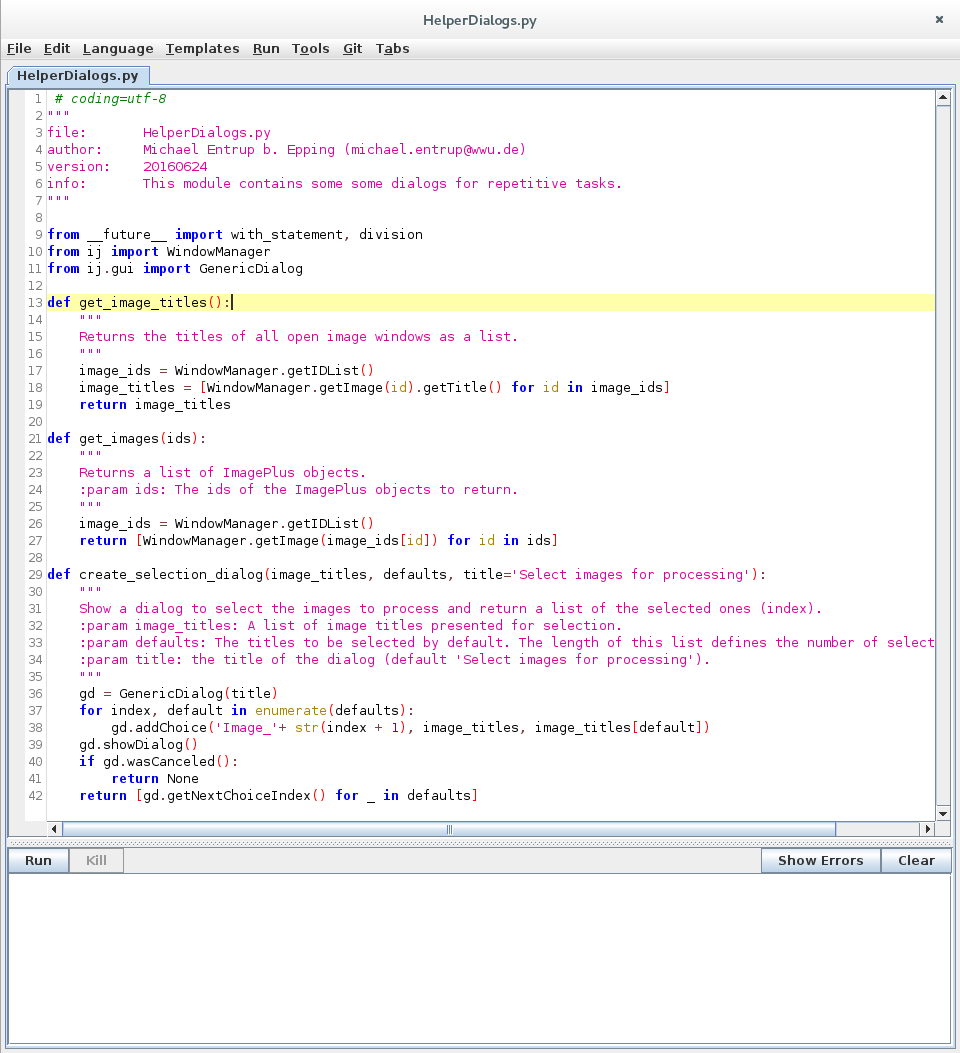
\includegraphics[width=1\linewidth]{Bilder/ImageJ_Script_Editor}
	\caption{Der Script-Editor von ImageJ. Zu sehen ist ein in Python geschriebenes Script. Durch die Syntaxhervorhebung ist der Code einfach zu lesen.}
	\label{fig:ImageJ_Script_Editor}
\end{figure}

ImageJ unterstützt eine Vielzahl von Script- und Programmiersprachen. Für alle unterstützten Sprachen eignet sich der Script-Editor \textbf{[Plugins > Macro > New]} zum Programmieren. Das Menü \textbf{[Language]} des Script-Editors führt alle verfügbaren Sprachen auf. Selektiert man eine der aufgelisteten Sprachen, wird die Syntax-Hervorhebung für diese aktiviert und ein Klick auf den Button \textbf{[Run]} führt das eingegebene Script mit dem passenden Interpreter aus.\footnote{Die Script-Sprachen müssen nicht kompiliert werden und können somit direkt innerhalb von Java ausgeführt werden (vergleiche \url{https://en.wikipedia.org/wiki/Interpreter_(computing)}).}
Abbildung \ref{fig:ImageJ_Script_Editor} zeigt den Script-Editor, welcher Python-Code auf Grund der Syntaxhervorhebung farblich darstellt.

Das Schreiben eines Scriptes ähnelt eher dem Entwickeln eines Java-Plugins, als dem Erstellen eines Macros. Es besteht voller Zugriff auf die Programmierschnittstelle von ImageJ und die installierten Bibliotheken (zum Beispiel Apache Commons Math).\footnote{Im Englischen \textit{\textbf{A}pplication \textbf{}Programming \textbf{I}nterface}, abgekürzt als \textbf{API}.}
Damit man darauf zugreifen kann, muss man jedoch einen Import eines Paketes, beziehungsweise einer Klasse ausführen. In Python wird beispielsweise \texttt{from ij import IJ} verwendet, um die Klasse \texttt{IJ} aus dem Paket \texttt{ij} zu importieren. Mit \texttt{IJ.run(imp, ''Gaussian Blur...'', ''sigma=5'')} kann man anschließend eine Funktion von ImageJ aufrufen, wie es in einem ImageJ-Macro mit \texttt{run(''Gaussian Blur...'', ''sigma=5'')} möglich ist. Der zusätzliche Parameter \texttt{imp} ist dabei eine Variable, die auf ein \texttt{ImagePlus}-Objekt verweist. Dieses \texttt{ImagePlus}-Objekt repräsentiert das Bild, auf das die Operation angewendet werden soll. Der Variable \texttt{imp} kann man auf verschiedene Weisen ein Bild zuweisen. Eine Möglichkeit ist die Verwendung von \texttt{imp = IJ.open(''Pfad/zur/Datei'')}\footnote{Statt einem Pfad kann man auch eine URL angeben, um ein Bild aus dem Internet zu laden. Wird Die Methode ohne Parameter aufgerufen, kann der Nutzer die Datei selber auswählen.}, womit man eine Datei vom lokalen Dateisystem lädt.

Mit dem Macro-Recorder kann man außerdem Befehle für Script-Sprachen und Java aufnehmen\footnote{Zur Auswahl stehen neben \textbf{Macro}, \textbf{JavaScript}, \textbf{BeanShell} und \textbf{Java} (Stand: 29.06.2016).}. Am wichtigsten ist jedoch die API-Dokumentation von ImageJ, die man unter \url{https://imagej.nih.gov/ij/developer/api/} findet. Diese Website wird automatisch aus dem JavaDoc von ImageJ generiert und listet sämtliche Klassen mit allen enthaltenen Methoden auf.\footnote{Leichter zu merken ist \url{http://javadoc.imagej.net/}, wo man die Dokumentation zu fast allen Projekten findet, die mit ImageJ in Verbindung stehen.} Außerdem kann der Sourcecode von ImageJ sich als hilfreich erweisen. Über die URL \url{https://imagej.nih.gov/ij/developer/source/} ruft man diesen im Browser auf. Viele Funktionen von ImageJ sind so implementiert, dass sie das Ergebnis einer Berechnung als Bild anzeigen (zum Beispiel die Kreuzkorrelation). Ein Blick in den Sourcecode von \texttt{FFTMath}\footnote{\url{https://imagej.nih.gov/ij/developer/source/ij/plugin/FFTMath.java.html}} verrät, wie man mit Hilfe der \textit{Fast Hartley Transform} (\texttt{FHT})\footnote{\url{https://imagej.nih.gov/ij/developer/source/ij/process/FHT.java.html}} in wenigen Schritten eine Kreuzkorrelation durchführt, deren Ergebnis als ein \texttt{ImagePlus}-Objekt vorliegt.

\subsection*{Python Grundlagen für ImageJ}\label{append:ImageJ-Python}

Mit EFTEMj-pyLib und EFTEMj-pyScripts enthält EFTEMj diverse Scripte für ImageJ, welche die Auswertung von ESI Aufnahmen erleichtern. Zu den Scripten gehören eine Driftkorrektur und diverse Scripte zur Berechnung von Jump-Ratio- und Element-Verteilungs-Bildern. Da der Quellcode zu umfangreich ist, um ihn hier abzudrucken, soll auf das Repository bei Github verwiesen werden, welches über die URL \url{https://github.com/m-entrup/EFTEMj} zu erreichen ist.

Bei den Scripten in EFTEMj-pyLib und EFTEMj-pyScripts wird Python verwendet, da diese Programmiersprache besonders leicht zu erlernen ist. Außerdem ist der Code sehr gut zu lesen, da in Python Code-Blöcke durch das Einrücken und nicht durch geschwungene Klammern definiert werden. Python-Code ließt sich außerdem viel eher wie natürliche Sprache, da zum Beispiel das Schlüsselwort \texttt{not} zum Negieren verwendet wird und nicht das Ausrufungszeichen.

\subsubsection[ImageJ verwendet Jython 2.5.3]{ImageJ verwendet Jython 2.5.3\footnote{Stand: 29.06.2016}}

Python ist eine Interpreter-Sprache und benötigt somit ein Programm, welches den Code ausführt. Der meist genutzte Interpreter ist CPython, welcher in C geschrieben ist. Für Java existiert der Interpreter Jython, welcher in ImageJ in der Version 2.5.3 enthalten ist. Das bedeutet, dass noch nicht alle Funktionen verfügbar sind, die Python in der aktuellen Version 2.7.x bietet\footnote{Python besitzt zwei aktuelle Versionen. Da viele Projekte auf Version 2.7.x basieren, wird diese parallel zu Version 3.4.x noch mit Updates versorgt.}. Eine große Einschränkung ist dieser Versions-Rückstand nicht.

Leider muss man in Jython auf viele Python-Bibliotheken verzichten. NumPy, matplotlib und viele mehr sind in C geschrieben und lassen sich dadurch nicht direkt in Jython importieren.

\subsubsection{Importieren von selbst geschriebenen Modulen}\label{append:Python-Module}

Damit die modularisierte Drifkorrektur funktioniert, muss das Haupt-Script die benötigten Module finden. Scripte werden bei ImageJ im Ordner \texttt{plugins/Scripts/} gespeichert. Unterordner bestimmen dabei, in welchem Menü das Script angezeigt wird. So sorgt der Pfad \texttt{plugins/Scripts/Plugins/Utilities/Record\_Desktop.py} dafür, dass im Menü \textbf{[Plugins > Utilities]} der Eintrag \textbf{[Record Desktop]} erscheint. Der Unterstrich im Dateinamen ist wichtig, damit das Script im Menü angezeigt wird. Beim Menüeintrag werden Unterstriche durch Leerzeichen ersetzt und die Dateiendung wird entfernt. Dateien, die keinen Unterstrich enthalten, werde nicht angezeigt. Sie können jedoch als Modul in anderen Scripten geladen werden. Dazu muss man jedoch die Variable \texttt{sys.path} um den Pfad zum Script erweitern. Einfacher ist es, wenn man ein Package\footnote{Ein Package ist ein Ordner der Python-Dateien (Module) enthält, wobei die Datei \texttt{\_\_init\_\_.py} unbedingt erforderlich ist.} im Ordner \texttt{jars/Lib} ablegt. Dieser Pfad ist schon in \texttt{sys.path} enthalt, weshalb Jython dort nach Modulen sucht.

Bei EFTEMj-pyLib und EFTEMj-pyScripts werden die einzelnen Scripte außerdem in einer JAR-Datei\footnote{Dabei handelt es sich im Prinzip um eine ZIP-Datei} verpackt. Dies dient dazu die vielen Script-Datein einfacher über eine ImageJ Update-Site zu verteilen. \texttt{EFTEMj-pyLib.jar} enthält das Python-Modul EFTEMj\_pyLib und wird im Ordner \texttt{jars/Lib} abgelegt. Dadurch kann man in einem Python-Script mit Hilfe von \texttt{import EFTEMj\_pyLib} das Modul importieren und die enthaltenen Scripte nutzen. \texttt{EFTEMj-pyScripts\_.jar} enthält einzelne Scripte, die ImageJ im Menü \textbf{[Plugins > EFTEMj]} anzeigt. Damit dies funktioniert, muss innerhalb der JAR-Datei die zuvor beschriebene Verzeichnisstruktur eingehalten werden. Der Pfad \texttt{/scripts/Plugins/EFTEMj/ESI/Calculate\_Jump-ratio.py} sorgt dafür, dass im Menü \textbf{[Plugins > EFTEMj > ESI]} der Eintrag \textbf{[Calculate Jump-ratio]} erscheint. \texttt{EFTEMj-pyScripts\_.jar} wird dazu im Ordner \texttt{plugins} abgelegt\footnote{In neueren Versionen von ImageJ (ab 1.51.?) ist es auch möglich \texttt{EFTEMj-pyScripts\_.jar} in \texttt{jars} abzulegen.}.

\section{Python-Scripte zur Auswertung von ESI Daten} \label{append:ESI-Scripte}

Dieser Abschnitt beschreibt diverse in Python geschriebene Scripte, welche Teil von EFTEMj sind. Den Code vollständig zu beschreiben würde den Umfang dieser Arbeit unnötig erhöhen. Es wird deshalb nur grob skizziert, wie vorgegangen wird und welche Auswirkungen das auf die Implementierung hat. Der vollständige Code ist im zugehörigen Repository bei GitHub finden, welches über die URL \url{https://github.com/m-entrup/EFTEMj} zu erreichen ist.

In Abschnitt \ref{append:ImageJ-Python} wurde die Nutzung von Python-Modulen in ImageJ beschrieben. Für die Auswertung von ESI Daten wird davon Gebrauch gemacht. Die Programmlogik ist in Module ausgelagert, die sich wiederverwenden lassen.

Die Driftkorrektur ist ein gutes Beispiel für die Verwendung von Modulen. Das Script \texttt{CorrectDrift.py} enthält Funktionen, um die Drift zu bestimmen, die zur Korrektur notwendigen Verschiebungsvektoren zu ermitteln und anschließend die Verschiebung durchzuführen. Die Bestimmung der Drift lässt sich dabei mit zwei verschiedenen Methoden durchführen. Mit Hilfe der Kreuzkorrelation bestimmt das Script \texttt{CrossCorrelation.py} die Verschiebung von zwei Bildern zueinander. Mit dem Script \texttt{pySIFT.py} steht eine Implementierung des Scale-invariant feature transform (SIFT) Algorithmus zur Verfügung, mit dessen Hilfe ebenfalls die Verschiebung von zwei Bildern zueinander bestimmt werden kann. SIFT wurde von Henriette Merkel auf die Eignung zur Driftkorrektur von TEM-Bildern untersucht. Die Ergebnisse können in ihrer Bachelorarbeit nachgelesen werden \cite{merkel_merkmalsbasierte_2016}. Die Driftkorrektur kann durch den modularen Aufbau sehr einfach um weitere Methoden zur Detektion der Drift erweitert werden.

Auch die gesamte Driftkorrektur ist so aufgebaut, dass sie in möglichst vielen Scripten verwendet werden kann. Der Aufruf von 

\texttt{corrected\_image\_list = CorrectDrift.get\_corrected\_images(limage\_list)}

genügt, um eine Liste von Bildern zu korrigieren. Mit dem optinalen Parameter \texttt{mode} kann man von SIFT auf Kreuzkorrelation umschalten. Da die Verwendung von SIFT zur Detektion von Drift fast nur Vorteile gegenüber der Verwendung von Kreuzkorrelation hat, ist SIFT die als Standard genutzte Methode.

\subsection*{Jump-Ratio Bilder berechnen}\label{append:Jump-Ratio-Script}

Um eine Jump-Ratio-Map zu berechnen, genügt eine Division des Post-edge Bilders durch das Pre-edge Bild. Dazu dient bei ImageJ der \textit{ImageCalculator}.\footnote{\url{https://imagej.nih.gov/ij/docs/guide/146-29.html\#toc-Subsection-29.13}} Auf Grund von Drift ist das erhaltene Ergebnis meist nicht sehr überzeugend, wie in Abbildung \ref{fig:Jump-ratio-noDK} zu sehen ist. Es sind Strukturen zu erkennen, die eigentlich nicht vorhanden sind. Im Vergleich zur Jump-ratio-Map, mit vorheriger Korrektur der Drift (siehe Abbildung \ref{fig:Jump-ratio-DK}), sind die Unterschiede gut sichtbar. Letztlich genügen drei Befehle, um eine Driftkorrektur auszuführen und eine Jump-Ratio-Map zu erzeugen. Diese drei Befehle sind in Listing \ref{lst:Jump-Ratio} aufgeführt. Die ersten drei Zeilen zeigen die Importe, die notwendig sind, um die zu verwendenden Befehle zu laden. Der erste Befehl führt die Driftkorrektur aus, wobei sich der eigentliche Programmcode im Modul \texttt{CorrectDrift} befindet. Als Eingabe dient ein Tuple aus zwei Bildern und ein String mit der zu verwendenden Methode. Das Ergebnis ist ein Stack aus zwei Bildern, der in Zeile 8 zu einer Liste umgewandelt wird. Da die Länge der Liste bekannt ist, können wird die beiden Einträge direkt in die Variablen \texttt{img1} und \texttt{img2} entpacken. In Zeile 9 wird der \textit{ImageCalculator} mit den Parametern \texttt{Divide} und \texttt{create} aufgerufen, womit \texttt{img2} durch \texttt{img1} geteilt wird und für das Ergebnis ein neues Bild erzeugt wird, welches wir der Variable \texttt{img\_ratio} zuweisen.

Das eigentliche Script ist mit fast 80 Zeilen Code wesentlich umfangreicher, da der Benutzer einen \textit{GenericDialog} präsentiert bekommt, um die zu verarbeitenden Bilder, sowie die zu verwendende Methode zur Detektion der Drift zu wählen. Außerdem wird die Darstellung der Jump-Ratio-Map unter Berücksichtigung von Mittelwert und Standardabweichung optimiert. Wichtig ist dabei, dass nur die Darstellung der Gleitkommazahlen als 256 Graustufen angepasst wird. Die eigentlichen Werte werden von dieser Optimierung nicht verändert.

\begin{figure}
	\centering
	\subfloat[Jump-ratio-Map, erstellt ohne Korrektur der Drift.]{ %
		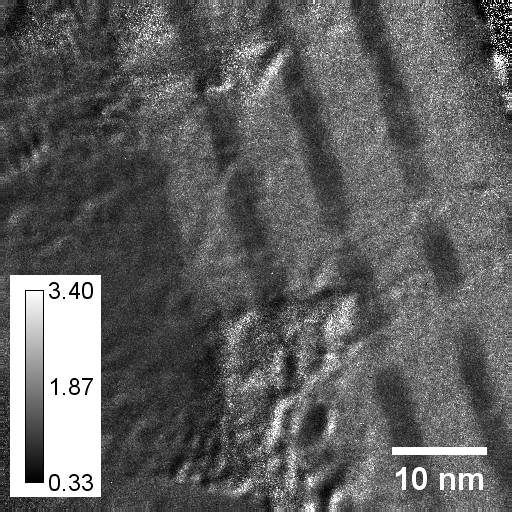
\includegraphics[width=.45\textwidth]{Bilder/Jump-ratio-Fe-noDK}
		\label{fig:Jump-ratio-noDK}
	}
	\qquad
	\subfloat[Jump-ratio-Map, erstellt nach Korrektur der Drift mit Hilfe von SIFT.]{ %
		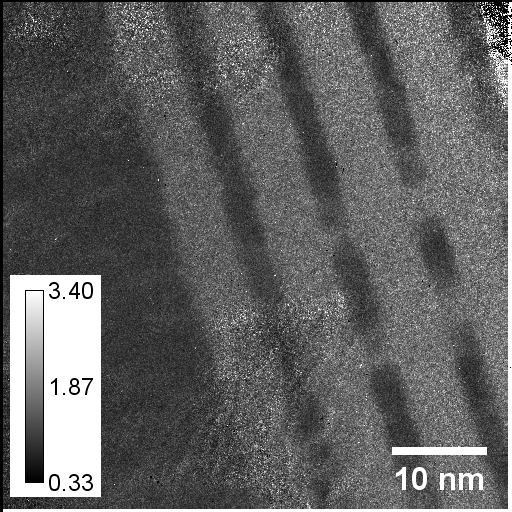
\includegraphics[width=.45\textwidth]{Bilder/Jump-ratio-Fe-DK}
		\label{fig:Jump-ratio-DK}
	}
	\caption[Eine Korrektur der Drift ist essenziell um richtige Ergebnisse bei der Jump-ratio-Methode zu erhalten.]{Eine Korrektur der Drift ist essenziell um richtige Ergebnisse zu erhalten. \subref{fig:Jump-ratio-noDK} zeigt welche Auswirkung eine Drift von \SI{0,9}{nm} auf die Jump-rati-Map hat. \subref{fig:Jump-ratio-DK} zeigt im Vergleich dazu das Ergebnis nach erfolgreicher Korrektur der Drift.}
	\label{fig:Jump-ratio-Drift}
\end{figure}

\begin{figure}
	\begin{lstlisting}[language=Python,caption={Die wichtigsten drei Zeilen Code bei der Berechnung der Jump-Ratio-Map.},label={lst:Jump-Ratio}]
	from EFTEMj_pyLib import CorrectDrift
	from EFTEMj_pyLib import Tools
	from ij.plugin import ImageCalculator
	
	corrected_stack = CorrectDrift.get_corrected_stack((img1_in, img2_in),
	mode='SIFT'
	)
	img1, img2 = Tools.stack_to_list_of_imp(corrected_stack)
	img_ratio = ImageCalculator().run('Divide create', img2, img1)
	img_ratio.show()
	\end{lstlisting}
\end{figure}

\subsection*{Die relative Dicke der Probe bestimmen} \label{append:Log-Ratio-Script}

Analog zur Berechnung einer Jump-Ratio-Map lässt sich die relative Dicke einer Probe bestimmen. Dazu werden zwei Bilder benötigt: Das erste Bild wird ohne Spaltblende in der energiedispersiven Ebene aufgenommen. Somit tragen alle Elektronen zum Bild bei ($I_0$). Zum zweiten Bild tragen nur die Elektronen des ZLP bei ($I_\mathrm{G}$). Es wird entsprechend eine Spaltblende in der energiedispersiven Ebene verwendet. Mit Hilfe der Gleichung 

\begin{align}
\frac{t}{\lambda} = \log\left(\frac{I_\mathrm{G}}{I_0}\right)
\end{align}

berechnet man anschließend Pixel für Pixel die relative Dicke $^t/_\lambda$, wobei $t$ die absolute Dicke darstellt und $\lambda$ die freie Weglänge der Elektronen in der Probe ist. Eine Herleitung dieser Gleichung ist zum Beispiel in \textit{Transmission Electron Microscopy and Diffractometry of Materials} von B.\,Fultz und J.\,M.\,Howe zu finden \cite[S.\ 175ff]{fultz_transmission_2008}. Die wichtigsten Befehle sind in Listing \ref{lst:relative_Dicke} aufgeführt. Im Vergleich zu Listing \ref{lst:Jump-Ratio} gibt es eine entschiedene Änderung: In Zeile 10 wird für jeden Pixel des Bildes \texttt{img\_ratio} der Logarithmus berechnet. Analog zur Jump-Ratio-Map gibt das Listingen nur die wichtigsten Befehle wieder. Das Vollständige Script umfasst ein Vielfaches an Code, um dem Benutzer die Auswahl der Bilder, sowie der zur Driftkorrektur verwendeten Methode mit Hilfe einer grafischen Oberfläche zu ermöglichen.

\begin{figure}
	\begin{lstlisting}[language=Python,caption={Die wichtigsten drei Zeilen Code bei der Berechnung der relativen Dicke.},label={lst:relative_Dicke}]
	from EFTEMj_pyLib import CorrectDrift
	from EFTEMj_pyLib import Tools
	from ij.plugin import ImageCalculator
	
	corrected_stack = CorrectDrift.get_corrected_stack((img_G_in, img_0_in),
	mode='SIFT'
	)
	img_G, img_0 = Tools.stack_to_list_of_imp(corrected_stack)
	img_ratio = ImageCalculator().run('Divide create', img_G, img_0)
	IJ.run(img_ratio, "Log", "")
	img_ratio.show()
	\end{lstlisting}
\end{figure}

\begin{figure}
	\centering
	\subfloat[Relative Dicke, erstellt ohne Korrektur der Drift.]{ %
		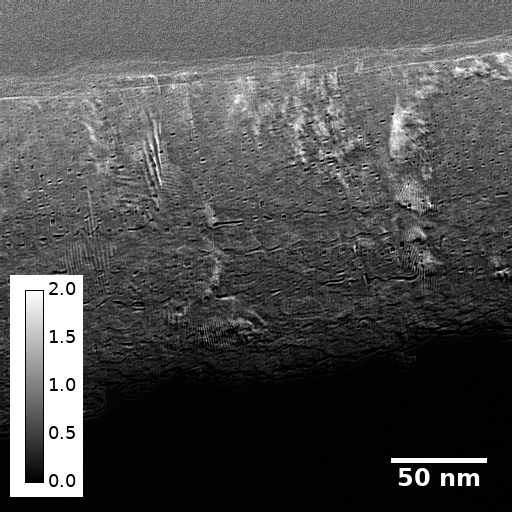
\includegraphics[width=.45\textwidth]{Bilder/rel-Dicke-noDK}
		\label{fig:rel-Dicke-noDK}
	}
	\qquad
	\subfloat[relative Dicke, erstellt nach Korrektur der Drift mit Hilfe von SIFT.]{ %
		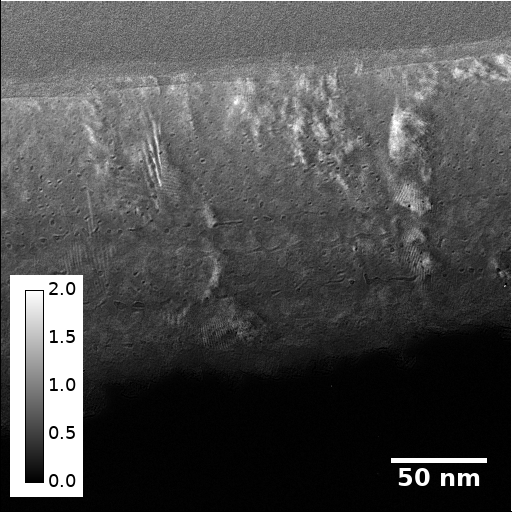
\includegraphics[width=.45\textwidth]{Bilder/rel-Dicke-DK}
		\label{fig:rel-Dicke-DK}
	}
	\caption[Eine Korrektur der Drift ist essenziell um richtige Ergebnisse bei der Bestimmung der relativen Dicke zu erhalten.]{Eine Korrektur der Drift ist essenziell um richtige Ergebnisse zu erhalten. \subref{fig:rel-Dicke-noDK} zeigt welche Auswirkung eine Drift von \SI{1,1}{nm} auf die Map der relativen Dicke hat. \subref{fig:rel-Dicke-DK} zeigt im Vergleich dazu das Ergebnis nach erfolgreicher Korrektur der Drift.}
	\label{fig:rel-Dicke}
\end{figure}

In Abbildung \ref{fig:rel-Dicke} ist die Map der relativen Dicke an einem Beispiel gezeigt. Wie schon bei der Jump-Ratio-Map führt eine erfolgreiche Korrektur der Drift zu einer deutlichen Verbesserung des Ergebnisses.

\section{Weitere Beispiel-Scripte}

\subsection*{Ein EEL Spektrum auslesen}

In Abschnitt 1.3 der Dissertation wird beschrieben, wie bei einem modernen TEM das EEL Spektrum aus der Parrallel-EELS-Aufnahme extrahiert wird. Dieser Schritt der Datenverarbeitung wird normalerweise von der Software durchgeführt, mit der man die Kamera des Mikroskops ansteuert. Das aufgenommene Bild wird somit als eindimensionaler Datensatz abgespeichert, der die Intensität in Abhängigkeit vom Energieverlust enthält.

Das aufgezeichnete Bild lässt sich auch speichern und mit ImageJ verarbeiten. 

% TODO: Script von JS nach Py portieren und Abschnitt fertigstellen.
% Dieser Abschnitt soll das folgende Script behandeln:
% Dissertation/Auswertungen/Erläuterung von EELS/createFig_EELS-Aufzeichnung.js
% Das Script muss noch modifiziert werden.
% Wahrscheinlich sollte ich es nach Python portieren.

\subsection*{Elemental-Mapping mit der 3-Fenster-Methode}

% TODO: Beschreibung von Elemental_mapping_(3-window).py mit Zitat von Kohl & Berger.

\clearpage

\bibliographystyle{../myamsalpha}
\bibliography{../Literatur}

\end{document}